\documentclass[conference]{IEEEtran}
\IEEEoverridecommandlockouts
\usepackage{cite}
\usepackage{amsmath,amssymb,amsfonts}
\usepackage{algorithmic}
\usepackage{graphicx}
\usepackage{textcomp}
\usepackage{xcolor}
\usepackage{booktabs}
\usepackage{multirow}
\graphicspath{{figures/}}
\def\BibTeX{{\rm B\kern-.05em{\sc i\kern-.025em b}\kern-.08em
    T\kern-.1667em\lower.7ex\hbox{E}\kern-.125emX}}
\begin{document}

\title{Multi-Agent Lane Merging via Policy Distillation:\\
Interaction-Aware Planning with Heterogeneous Driver Types}

\author{\IEEEauthorblockN{Nathan McNaughton}
\IEEEauthorblockA{\textit{Dept. of Electrical Engineering and Computer Sciences} \\
\textit{University of California, Berkeley}\\
nathanmc03@berkeley.edu}
\and
\IEEEauthorblockN{Shanaya Malik}
\IEEEauthorblockA{\textit{Dept. of Electrical Engineering and Computer Sciences} \\
\textit{University of California, Berkeley}\\
shanaya\_malik@berkeley.edu}
}

\maketitle

\begin{abstract}
Lane merging is one of the most challenging highway maneuvers for autonomous
vehicles, requiring real-time coordination with surrounding drivers who exhibit
diverse and often unpredictable behavioral tendencies.
Existing interaction-aware planners address two-agent scenarios or assume
homogeneous driver models, leaving a gap for deployable policies that reason
jointly over heterogeneous, non-communicating agents in multi-vehicle merges.
We present a three-stage distillation pipeline that converts a multi-agent
model predictive control (MPC) expert---which plans via iterative best response
over drivers modeled with three heterogeneous archetypes grounded in social
value orientation theory---into a fast, deployable neural policy via behavioral
cloning followed by proximal policy optimization (PPO) fine-tuning.
The approach requires no inter-vehicle communication and operates entirely from
onboard observations.
Evaluated across four traffic compositions in the Highway-Env merge-v0 simulator,
our PPO policy achieves 96\% merge success and 0\% crash rate on the default
traffic mix, compared to 92\% and 2\% for the MPC expert it was distilled from.
The distilled policy operates at 19.6~m/s---2.5 times faster than the expert---
while maintaining a mean minimum time-to-collision of 15.1~s, approximately 31
times the expert's 0.48~s, demonstrating that closed-loop reinforcement learning
recovers both speed and safety margins lost at the expert imitation stage.
\end{abstract}

\begin{IEEEkeywords}
autonomous vehicles, lane merging, model predictive control, behavioral cloning,
proximal policy optimization, driver heterogeneity, multi-agent planning
\end{IEEEkeywords}

% =============================================================================
\section{Introduction}
% =============================================================================

Lane merging is a deceptively difficult task. At the moment of merge, an
autonomous vehicle (AV) must predict how several surrounding drivers will react
to its own trajectory, adjust that trajectory in real time, and complete the
maneuver before the available gap closes---all without explicit communication
with any other vehicle. Human drivers accomplish this through a mix of
anticipation, signaling, and social negotiation; replicating this capability in
a principled, deployable system remains an open problem in autonomous driving.

The difficulty is compounded by two properties of real traffic. First, the
problem is inherently \emph{multi-agent}: the ego vehicle's trajectory affects
every surrounding vehicle, and those vehicles' reactions are coupled to each
other, not just to the ego. Second, drivers are \emph{heterogeneous}: a cautious
driver holding a large gap, a normal driver following standard spacing, and an
aggressive driver minimizing headway all require qualitatively different
negotiation strategies from the AV. A planner that ignores either property risks
being overly conservative (stalling on the ramp) or overly risky (forcing its
way into an occupied gap).

Prior work addresses these challenges only partially.
Sadigh et al.\ \cite{sadigh2016planning} formalize AV-human interaction as a
Stackelberg game and derive a planner that anticipates how its own trajectory
alters the human driver's best response---a foundational contribution, but
restricted to \emph{two agents}.
Zhang et al.\ \cite{zhang2025multiagent} extend game-theoretic merging to
multiple vehicles via branch MPC, but their driver model is binary
(Assert/Yield), losing the continuous behavioral spectrum observed in real
traffic.
Schwarting et al.\ \cite{schwarting2019social} provide a rigorous taxonomy of
driver types via social value orientation (SVO), defining cautious, normal, and
aggressive archetypes with distinct Intelligent Driver Model (IDM)
\cite{treiber2000congested} parameterizations---but the work stops short of a
merging planner or a deployable policy.
Zhou et al.\ \cite{zhou2022marl} train a multi-agent reinforcement learning
(MARL) policy for cooperative lane changing in mixed traffic, achieving
strong results, but their approach assumes connected vehicles sharing parameters
and a single politeness coefficient, rather than distinct non-communicating
archetypes.
No existing work combines multi-agent interaction-aware planning,
heterogeneous non-communicating drivers, and a deployable distilled policy for
the lane merging problem.
A schematic of the simulation scenario is shown in Fig.~\ref{fig:scenario}.

We close this gap with the following contributions:

\begin{enumerate}
    \item \textbf{Multi-agent heterogeneous MPC expert.} We extend Sadigh et
    al.'s iterative best-response (IBR) framework from two agents to $N$
    non-ego vehicles, each independently assigned one of three IDM-parameterized
    driver archetypes (cautious, normal, aggressive) grounded in Schwarting et
    al.'s SVO taxonomy. The expert scores candidate ego trajectories against
    jointly-predicted NPC responses, planning over four traffic compositions.

    \item \textbf{Three-stage distillation pipeline.} We convert the MPC expert
    into a deployable neural policy via (i) dataset generation from 74,128 clean
    MPC-labeled transitions, (ii) behavioral cloning (BC) into a 4-layer MLP,
    and (iii) PPO fine-tuning warm-started from the BC weights. The pipeline
    addresses distribution shift and reward hacking through systematic reward
    shaping and environment wrapper design.

    \item \textbf{Empirical analysis of multi-agent coupling.} We introduce an
    independent-baseline planner that applies Sadigh et al.'s two-agent IBR
    naively---predicting each NPC as if the others were absent---and compare
    it against the full multi-agent MPC. The near-identical merge success rates
    (90\% vs.\ 92\%) reveal that in this scenario the primary performance gain
    comes from closed-loop RL, not from modeling inter-vehicle interactions,
    with important implications for when multi-agent coupling is worth its
    computational cost.
\end{enumerate}

Our PPO policy achieves 96\% merge success, 0\% crashes, and a mean speed of
19.6~m/s across 50 held-out episodes on the default traffic mix. It maintains
these results with 0\% crashes across all four traffic compositions despite
being trained exclusively on the default mix, demonstrating robustness to
out-of-distribution traffic. The codebase is available at
\texttt{https://github.com/shanayamalik/cs290-sp26}.

\begin{figure}[t]
  \centering
  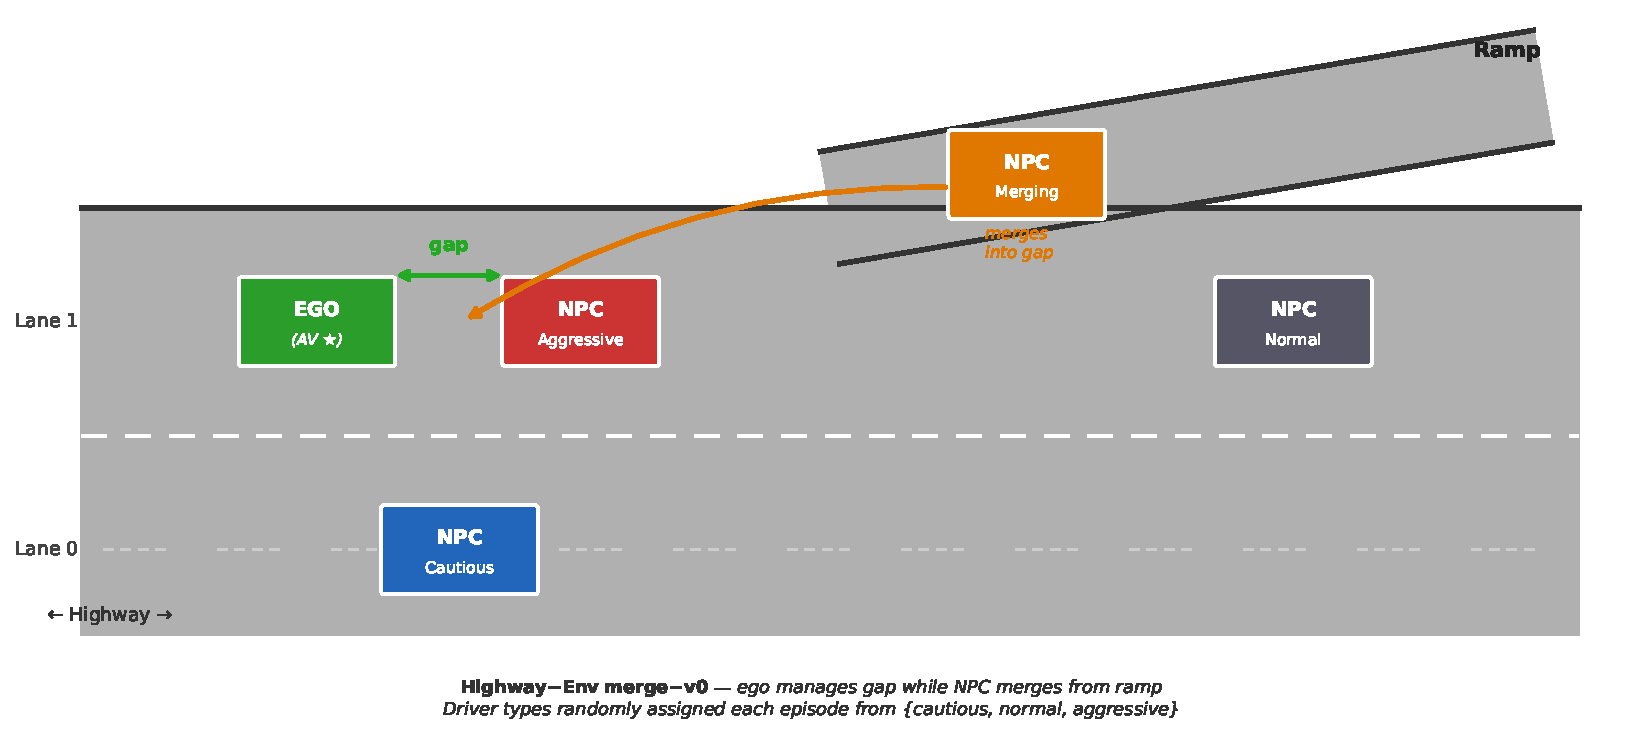
\includegraphics[width=\columnwidth]{figures/merge_diagram}
  \caption{Highway-Env \texttt{merge-v0} scenario. The ego vehicle (green,
    Lane~1) must manage a gap for the merging NPC (orange, ramp) while
    avoiding a heterogeneous mix of NPC drivers (red: aggressive, blue:
    cautious, gray: normal) in both highway lanes.
    Driver types are independently assigned at the start of each episode.}
  \label{fig:scenario}
\end{figure}

The remainder of the paper is organized as follows. Section~\ref{sec:related}
situates our work within the existing literature. Section~\ref{sec:methods}
presents the formal problem definition, driver model, reward structure, and
each stage of the pipeline. Section~\ref{sec:results} reports experimental
results. Section~\ref{sec:discussion} interprets the findings, discusses
limitations, and outlines future directions. Section~\ref{sec:contributions}
summarizes individual group contributions.

% =============================================================================
\section{Related Work}
\label{sec:related}
% =============================================================================

\textbf{Interaction-aware planning.}
Sadigh et al.\ \cite{sadigh2016planning} introduced the foundational framework
for interaction-aware AV planning by modeling the human driver as a rational
agent whose trajectory is a best response to the AV's own planned path.
Their Stackelberg game formulation---wherein the AV acts as the leader and
anticipates the follower's reaction when scoring its own trajectory
candidates---yields plans that actively shape human behavior rather than
treating it as fixed.
Our MPC expert directly extends this iterative best-response (IBR)
framework to a multi-vehicle setting: rather than one ego-human pair, we
maintain coupled predictions for all $N-1$ non-ego vehicles and iterate
their responses jointly.
The key departure is that Sadigh et al.\ study a single human driver;
applying IBR naively to each NPC in isolation---our independent baseline---
proves nearly as effective in terms of merge success, which motivates the
closed-loop RL stage as the primary source of performance gain.

\textbf{Multi-vehicle merging via game theory.}
Zhang et al.\ \cite{zhang2025multiagent} address multi-vehicle highway merging
through a combination of game-theoretic planning and branch MPC, achieving
strong results in a scenario structurally similar to ours.
Their work is the closest task-level comparison: both approaches plan over
multiple interacting vehicles at a merge point.
The principal gap is in the driver model.
Zhang et al.\ represent non-ego drivers with a binary Assert/Yield
parameterization, which captures dominance but collapses the continuous
behavioral spectrum present in real traffic.
We instead ground our three driver archetypes---cautious, normal, and
aggressive---in distinct IDM parameter sets \cite{treiber2000congested},
producing qualitatively different following behaviors (time headway ranging
from 1.0~s to 2.5~s, acceleration ceiling from 1.2 to 2.5~m/s$^2$).
Additionally, Zhang et al.\ do not produce a deployable policy; their
planner runs online at each timestep, while our pipeline distills the
expert into a neural network with sub-millisecond inference.

\textbf{Driver heterogeneity via social value orientation.}
Schwarting et al.\ \cite{schwarting2019social} provide the theoretical
grounding for our driver taxonomy.
They measure the social value orientation (SVO) angle $\phi$ of human
drivers in naturalistic data and show that the distribution is trimodal:
prosocial ($\phi \approx \pi/4$), individualistic ($\phi \approx 0$), and
competitive ($\phi \approx -\pi/4$) drivers each constitute a distinct
cluster.
We operationalize this taxonomy directly: our cautious archetype corresponds
to the prosocial cluster (low self-weight on forward progress, large time
headway), normal to individualistic (standard IDM reference values), and
aggressive to competitive (short headway, high acceleration).
The gap left by Schwarting et al.\ is twofold: their work characterizes
driver types from data but does not apply the taxonomy to the merging
planning problem, and it does not produce a policy of any kind.
Our work is, to our knowledge, the first to use the SVO framework as the
basis for driver models within an interactive merge planner.

\textbf{Learning reward functions from driver behavior.}
Huang et al.\ \cite{huang2021personalized} propose learning personalized
reward functions for individual drivers from observed trajectories via
inverse reinforcement learning (IRL).
Their feature-based reward structure $r = \theta^\top f(s, u)$, where
features encode forward progress, proximity cost, smoothness, and comfort,
is the same formalism we adopt for our ego reward and NPC planning
objectives.
The distinction is that Huang et al.\ \emph{learn} $\theta$ from data,
while we \emph{hand-define} the weight vectors based on the SVO taxonomy
and domain knowledge.
This is a deliberate simplification: hand-tuning allows us to guarantee
that the reward structure matches the intended behavioral archetype without
requiring rollout data from real human drivers of each type.
The limitation is that our weights may not accurately reflect real traffic;
replacing them with IRL-estimated weights from naturalistic driving datasets
is a natural direction for future work.

\textbf{Multi-agent reinforcement learning for lane changing.}
Zhou et al.\ \cite{zhou2022marl} train a MARL policy for cooperative lane
changing in mixed autonomy traffic, demonstrating that RL agents can learn
to coordinate smooth lane changes alongside human-modeled vehicles.
Their work is the closest methodological comparison to our PPO fine-tuning
stage.
However, several design choices differ in ways that matter for deployment.
First, Zhou et al.\ assume connected autonomous vehicles that share policy
parameters and communicate implicitly through a shared reward structure;
our AV plans \emph{unilaterally}, receiving no information from surrounding
vehicles beyond its onboard observation.
Second, they model driver heterogeneity through a single politeness
coefficient, whereas we assign each NPC a full set of IDM parameters
covering acceleration ceiling, braking limit, time headway, and standstill
gap.
Third, their policy is trained from scratch via MARL, while ours is
warm-started from a behavioral cloning initialization of an MPC expert,
which substantially accelerates convergence and avoids early-training
crashes that corrupt the replay buffer.

\textbf{Summary.}
No prior work simultaneously addresses all three properties of our
setting: (i) multi-agent interaction-aware planning that couples NPC
predictions across all vehicles, (ii) heterogeneous non-communicating
driver archetypes grounded in SVO theory with distinct IDM
parameterizations, and (iii) a deployable distilled policy produced
through a structured expert-to-RL pipeline.
Our contribution lies in the combination: the MPC expert provides safe,
interpretable training data; BC provides a warm start that avoids
early-training instability; and PPO fine-tuning recovers the speed and
safety margins that BC alone cannot achieve due to distribution shift.

% =============================================================================
\section{Methods}
\label{sec:methods}
% =============================================================================

Our approach consists of three stages: (1) an MPC expert that generates
interaction-aware demonstrations using iterative best response over
heterogeneous IDM drivers, (2) behavioral cloning that compresses these
demonstrations into a neural policy via supervised regression, and (3)
PPO fine-tuning that recovers closed-loop performance and generalizes
across traffic compositions.
We describe each stage in turn after formalizing the problem and the
driver model.

\subsection{Problem Formulation}

We consider a multi-agent highway merge scenario simulated in the
Highway-Env \texttt{merge-v0} environment \cite{leurent2018highway}.
The scene contains $N = 5$ vehicles: one controlled ego vehicle and four
non-player characters (NPCs).\footnote{Highway-Env's
\texttt{vehicles\_count=3} configuration parameter controls spawn
density rather than an exact headcount; the environment consistently
produces five vehicles in this setting.}
The ego occupies the upper highway lane and must maintain forward progress
while an NPC vehicle merges from a ramp lane; three additional NPCs occupy
the highway lanes ahead of and beside the ego.

\textbf{State and dynamics.}
Each vehicle $i$ has state $s_i = [x_i,\, y_i,\, v_{x,i}] \in \mathbb{R}^3$
representing longitudinal position, lateral position, and longitudinal speed.
The joint state at time $t$ is $S_t = (s_t^{(1)}, \ldots, s_t^{(N)})$.
The ego's action is $u_t = [a_t] \in [-1, 1]$, a normalized acceleration
command; steering is fixed at zero since the ego need not change lanes.
Ego dynamics follow:
\begin{align}
  v_{t+1} &= \text{clip}(v_t + \alpha\, u_t\, \Delta t,\; 0,\; 40), \label{eq:ego_v} \\
  x_{t+1} &= x_t + v_t\, \Delta t, \label{eq:ego_x}
\end{align}
where $\alpha = 5$~m/s$^2$ is the physical acceleration scale and
$\Delta t = 1.0$~s is the environment step duration (simulation frequency
15~Hz, policy frequency 1~Hz).
NPC dynamics are governed by the Intelligent Driver Model (IDM)
\cite{treiber2000congested} at a finer integration timestep of $\delta t = 0.1$~s,
with per-vehicle parameters determined by driver archetype (Section~\ref{sec:driver_het}).

\textbf{Observation space.}
The raw Highway-Env observation is $O \in \mathbb{R}^{5 \times 5}$:
five rows (ego $+$ four nearest vehicles) by five features
(presence, $x$, $y$, $v_x$, $v_y$), flattened to $\mathbb{R}^{25}$.
For behavioral cloning (BC) we augment this with two scalars---minimum
distance to any NPC ($d_{\min}$) and episode step count---yielding
$o^{\text{BC}} \in \mathbb{R}^{27}$.
For PPO fine-tuning we add a third scalar (ego speed), giving
$o^{\text{PPO}} \in \mathbb{R}^{28}$.
All observations are normalized to zero mean and unit variance using
statistics computed from the BC training dataset.

% ---------------------------------------------------------------------------
\subsection{Driver Heterogeneity}
\label{sec:driver_het}
% ---------------------------------------------------------------------------

\textbf{SVO taxonomy.}
Following Schwarting et al.\ \cite{schwarting2019social}, we characterize
driver behavior by a social value orientation (SVO) angle $\phi$ that
encodes the trade-off between self-interest and regard for others.
The SVO utility for driver $i$ is
\begin{equation}
  U_i(r_{\text{self}}, r_{\text{other}}) =
    r_{\text{self}} \cos\phi_i + r_{\text{other}} \sin\phi_i,
  \label{eq:svo}
\end{equation}
where $r_{\text{self}}$ and $r_{\text{other}}$ are the driver's own reward
and the average reward of surrounding vehicles.
Schwarting et al.\ identify three empirical clusters: prosocial
($\phi \approx \pi/4$), individualistic ($\phi \approx 0$), and competitive
($\phi \approx -\pi/4$).
We map these to three IDM-parameterized archetypes---\emph{cautious},
\emph{normal}, and \emph{aggressive}---whose parameters are summarized
in Table~\ref{tab:idm}.

\begin{table}[t]
  \caption{IDM parameters per driver archetype.
    $a_{\max}$: max acceleration; $b$: comfortable deceleration;
    $T$: desired time headway; $s_0$: minimum gap; $\delta$: velocity exponent.}
  \label{tab:idm}
  \centering
  \begin{tabular}{lcccccc}
    \toprule
    Archetype & SVO & $a_{\max}$ & $b$ & $T$ & $s_0$ & $\delta$ \\
              &     & (m/s$^2$) & (m/s$^2$) & (s) & (m) & \\
    \midrule
    Cautious   & prosocial      & 1.2 & 1.5 & 2.5 & 8.0 & 4 \\
    Normal     & individualistic & 1.5 & 2.0 & 1.5 & 2.0 & 4 \\
    Aggressive & competitive    & 2.5 & 4.0 & 1.0 & 1.5 & 4 \\
    \bottomrule
  \end{tabular}
\end{table}

\textbf{Traffic mixes.}
At the start of each episode, each NPC is independently assigned an archetype
by sampling from a predefined traffic composition.
We evaluate four mixes (Table~\ref{tab:mixes}): \texttt{default\_mix}
(60\% normal, 20\% cautious, 20\% aggressive), \texttt{all\_normal},
\texttt{cautious\_heavy} (${\sim}$50\% cautious), and
\texttt{aggressive\_heavy} (${\sim}$50\% aggressive).
Driver types are assumed known at planning time in the MPC and baseline;
online type estimation from observed trajectories is left as future work.

\begin{table}[t]
  \caption{Traffic mix compositions used for training and evaluation.}
  \label{tab:mixes}
  \centering
  \begin{tabular}{lccc}
    \toprule
    Mix & Normal & Cautious & Aggressive \\
    \midrule
    \texttt{default\_mix}      & 60\% & 20\% & 20\% \\
    \texttt{all\_normal}       & 100\% & 0\%  & 0\%  \\
    \texttt{cautious\_heavy}   & 40\% & 50\% & 10\% \\
    \texttt{aggressive\_heavy} & 40\% & 10\% & 50\% \\
    \bottomrule
  \end{tabular}
\end{table}

% ---------------------------------------------------------------------------
\subsection{Reward Functions}
% ---------------------------------------------------------------------------

We adopt the feature-based reward formalism of Huang et al.\ \cite{huang2021personalized}
and Sadigh et al.\ \cite{sadigh2016planning}:
\begin{equation}
  r(s_t, u_t;\, \theta) = \theta^\top f(s_t, u_t),
  \label{eq:reward}
\end{equation}
where $f: \mathcal{S} \times \mathcal{U} \to \mathbb{R}^6$ is a hand-crafted
feature vector and $\theta \in \mathbb{R}^6$ is a driver-type weight vector.
The six features are:
\begin{enumerate}
  \item \textbf{Forward progress}: $f_1 = v_x / v^*$, ego speed normalized
        by the desired highway speed $v^* = 30$~m/s.
  \item \textbf{Proximity penalty}: $f_2 = 1 / \max(d_{\min}^2, 0.1)$, a
        repulsive potential that grows as $1/d^2$ near surrounding vehicles,
        following Khatib \cite{khatib1986realtime}.
  \item \textbf{Smoothness}: $f_3 = -a^2$, penalizing large accelerations
        for comfort \cite{bae2020toward}.
  \item \textbf{Jerk}: $f_4 = -(\dot{a})^2 = -((a_t - a_{t-1})/\delta t)^2$,
        penalizing rapid changes in acceleration.
  \item \textbf{Collision}: $f_5 = \mathbf{1}[\text{collision}]$, an indicator
        that fires when any vehicle overlap is detected.
  \item \textbf{Lane deviation}: $f_6 = -(y - y^*)^2$, where $y^*$ is the
        target lane center. This feature is identically zero for the ego
        (which stays in its lane) and is zeroed in the weight vectors.
\end{enumerate}

Weight vectors $\theta$ encode the SVO taxonomy: cautious drivers weight
proximity heavily; aggressive drivers weight forward progress.
The collision weight $\theta_5 = -1000$ for all archetypes, dominating
any per-step gain: the maximum cumulative non-collision reward over a 50-step
horizon is at most $50 \times 0.9 = 45 \ll 1000$, ensuring that no
trajectory score can justify a crash.
Full weight vectors are given in Table~\ref{tab:weights}.

\begin{table}[t]
  \caption{Reward weight vectors $\theta$ per driver archetype.
    Features: $f_1$~=~forward progress, $f_2$~=~proximity,
    $f_3$~=~smoothness, $f_4$~=~jerk, $f_5$~=~collision, $f_6$~=~lane deviation.}
  \label{tab:weights}
  \centering
  \begin{tabular}{lrrrrrr}
    \toprule
    Archetype & $\theta_1$ & $\theta_2$ & $\theta_3$ & $\theta_4$ & $\theta_5$ & $\theta_6$ \\
    \midrule
    Cautious   &  0.2 & $-$2.0 & $-$0.5 & $-$0.3 & $-$1000 & 0.0 \\
    Normal     &  0.5 & $-$1.0 & $-$0.3 & $-$0.2 & $-$1000 & 0.0 \\
    Aggressive &  0.9 & $-$0.5 & $-$0.1 & $-$0.1 & $-$1000 & 0.0 \\
    \bottomrule
  \end{tabular}
\end{table}

% ---------------------------------------------------------------------------
\subsection{MPC Expert via Iterative Best Response}
% ---------------------------------------------------------------------------

The MPC expert selects the ego's action at each timestep by maximizing
predicted cumulative reward over a finite horizon, using iterative
best response (IBR) to couple NPC predictions \cite{sadigh2016planning}.

\textbf{NPC prediction.}
Given a nominal ego trajectory $\tau_{\text{ego}} = (s_0, s_1, \ldots, s_H)$,
the IBR procedure predicts each NPC's response by running IDM with that
vehicle's archetype parameters, treating the ego and other NPCs as lead
vehicles.
Iterating $K = 4$ rounds with convergence threshold $\epsilon = 0.1$
(max per-step position change in meters):
\begin{equation}
  \hat{\tau}_j^{(k+1)} = \text{IDM}\!\left(j \;\Big|\; \tau_{\text{ego}},\;
  \bigl\{\hat{\tau}_{i \neq j}^{(k)}\bigr\}\right), \quad k = 0, \ldots, K-1,
  \label{eq:ibr}
\end{equation}
initialized with straight-line constant-speed predictions
$\hat{\tau}_j^{(0)}$.
Non-convergence is expected with aggressive NPCs (short headway leads to
oscillation); in such cases the final iterate is used as a fallback.
The IDM integration uses $\delta t = 0.1$~s over a 5-second horizon.

\textbf{Action selection.}
We maintain $M = 50$ candidate ego action sequences, each consisting of
$W = 6$ acceleration waypoints interpolated to the full planning horizon
$H = 20$ steps.
Three structured candidates (constant speed, gentle braking at $-0.3$,
gentle acceleration at $+0.3$) are always evaluated alongside $M - 3$
random samples from $[-1, 1]^W$, ensuring reasonable coverage even when
random sampling is sparse.
The best-scoring sequence under \eqref{eq:reward} with $\theta = \theta_{\text{normal}}$
is selected; if all scores fall below a crash threshold of $-500$, a
fallback braking action $u = -0.5$ is returned.
Each MPC call takes approximately 12~ms, too slow for real-time deployment
at 100~Hz but sufficient for generating training data offline.

% ---------------------------------------------------------------------------
\subsection{Independent Planning Baseline}
% ---------------------------------------------------------------------------

To isolate the value of multi-agent coupling, we define an independent
planning baseline that applies Sadigh et al.'s two-agent IBR naively to
the multi-vehicle setting.
Rather than iterating responses jointly across all NPCs as in
\eqref{eq:ibr}, the baseline predicts each NPC $j$ independently:
\begin{equation}
  \hat{\tau}_j^{\text{ind}} = \text{IDM}\!\left(j \;\Big|\; \tau_{\text{ego}}\right),
  \label{eq:baseline}
\end{equation}
treating the other NPCs as absent when computing $j$'s response.
The ego then scores candidate trajectories against the union of these
independent predictions using the same sampling and scoring procedure as
the full MPC.
The difference between \eqref{eq:ibr} and \eqref{eq:baseline} is precisely
whether NPC-to-NPC interaction chains are modeled; comparing the two
directly measures how much multi-agent coupling contributes to performance.

% ---------------------------------------------------------------------------
\subsection{Behavioral Cloning}
% ---------------------------------------------------------------------------

The first learning stage distills the MPC expert into a neural policy via
supervised regression.
We minimize the mean squared error between policy outputs and MPC-labeled
actions:
\begin{equation}
  \theta^*_{\text{BC}} = \arg\min_{\theta} \frac{1}{N} \sum_{i=1}^{N}
  \bigl\|\pi_\theta(o_i) - u_i^{\text{MPC}}\bigr\|_2^2.
  \label{eq:bc}
\end{equation}

\textbf{Dataset.}
We generated 400 MPC episodes per traffic mix (1,600 total) and retained
only crash-free transitions, yielding $N = 74{,}128$ clean
$(o_i, u_i^{\text{MPC}})$ pairs distributed as: 18,629 (\texttt{all\_normal}),
18,346 (\texttt{default\_mix}), 18,630 (\texttt{cautious\_heavy}), and 18,523
(\texttt{aggressive\_heavy}).
Summary statistics for each split are given in Table~\ref{tab:dataset}.
During initial data collection, a sign error in the proximity reward
feature caused the MPC to treat closeness as attractive rather than
repulsive, contaminating approximately 65\% of transitions with
backwards-driving behavior.
After correcting the sign and adding a speed floor that prevents the ego
from reversing, the full dataset was regenerated from scratch.

\begin{table}[t]
  \caption{BC training dataset statistics per traffic mix
    (400 MPC episodes each, crash-free transitions only).}
  \label{tab:dataset}
  \centering
  \begin{tabular}{lcc}
    \toprule
    Mix & Clean transitions & Fraction of total \\
    \midrule
    \texttt{all\_normal}       & 18,629 & 25.1\% \\
    \texttt{default\_mix}      & 18,346 & 24.7\% \\
    \texttt{cautious\_heavy}   & 18,630 & 25.1\% \\
    \texttt{aggressive\_heavy} & 18,523 & 25.0\% \\
    \midrule
    Total                    & 74,128 & 100\% \\
    \bottomrule
  \end{tabular}
\end{table}

\textbf{Network architecture.}
The policy network $\pi_\theta$ is a 4-layer MLP:
$27 \to 256 \to 256 \to 128 \to 2$, with ReLU activations in the hidden
layers and a tanh output layer that enforces the $[-1, 1]$ action range.
The network has 106,114 trainable parameters.

\textbf{Training protocol.}
We train for 100 epochs with batch size 256, initial learning rate
$\eta = 10^{-3}$, and ReduceLROnPlateau scheduling (patience 5, factor 0.5).
The dataset is split 90/10 into training and validation sets.
Training and validation loss curves for all four mixes are shown in
Fig.~\ref{fig:bc_loss}.
The model trained on \texttt{default\_mix} alone is used as the BC
initialization for PPO fine-tuning, as it provides the best balance across
traffic conditions (Section~\ref{sec:results}).

\begin{figure}[t]
  \centering
  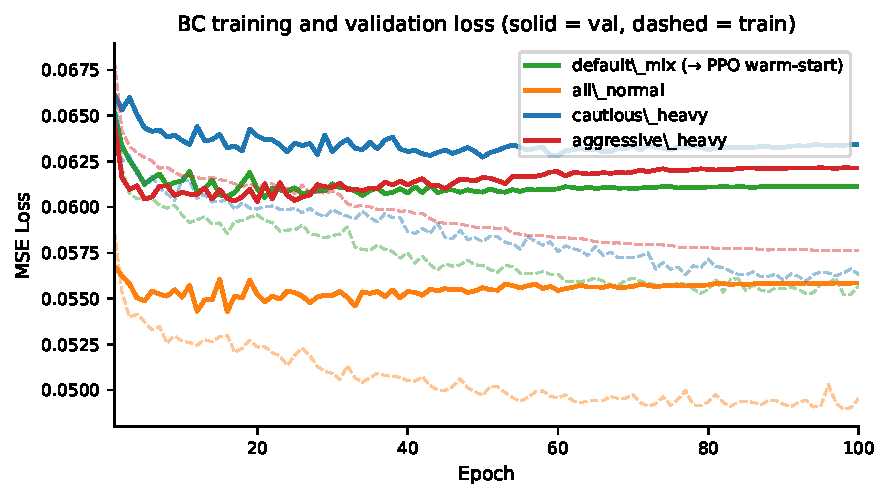
\includegraphics[width=\columnwidth]{figures/bc_loss}
  \caption{BC training (dashed) and validation (solid) MSE loss over 100
    epochs for each traffic mix.
    All mixes converge smoothly; \texttt{default\_mix} (green) is selected
    as the warm-start for PPO fine-tuning.}
  \label{fig:bc_loss}
\end{figure}

% ---------------------------------------------------------------------------
\subsection{PPO Fine-Tuning}
% ---------------------------------------------------------------------------

Behavioral cloning alone suffers from distribution shift: the BC policy
never recovers from states outside the expert's trajectory distribution.
We address this with proximal policy optimization (PPO)
\cite{schulman2017ppo}, fine-tuning from the BC warm start in a
closed-loop environment.

\textbf{Objective.}
PPO maximizes a clipped surrogate objective:
\begin{equation}
  \mathcal{L}^{\text{CLIP}}(\theta) = \mathbb{E}_t\!\left[\min\!\left(
    r_t(\theta)\, \hat{A}_t,\;
    \text{clip}(r_t(\theta), 1-\varepsilon, 1+\varepsilon)\, \hat{A}_t
  \right)\right],
  \label{eq:ppo}
\end{equation}
where $r_t(\theta) = \pi_\theta(a_t \mid o_t) / \pi_{\theta_{\text{old}}}(a_t \mid o_t)$
is the probability ratio and $\hat{A}_t$ is the generalized advantage estimate.

\textbf{Warm start.}
The PPO actor is initialized from the BC weights.
Because PPO uses a 28-dimensional observation (BC uses 27), we copy the
BC weights into the first 27 input columns of the first linear layer and
zero the 28th column, so the network initially behaves identically to BC.
The log-standard deviation is initialized to $-1.0$ to produce a narrow
initial action distribution close to the deterministic BC policy.

\textbf{Reward shaping.}
The environment reward is augmented with: a speed bonus
($+0.04 \cdot \min(v, 20)$~m/s), a forward progress bonus
($+0.03 \cdot \max(\Delta x, 0)$), a time penalty ($-0.05$ per step),
a speed clamping penalty ($-1.0$ when the speed floor fires), an
overspeed penalty ($-0.15 \cdot (v - 20)$ for $v > 20$~m/s), milestone
bonuses ($+5.0$ per 50~m of novel forward progress), a completion bonus
($+20.0$ at episode success), and a shaped truncation reward
($+0.05 \cdot \max(x - x_0, 0)$ at step limit).
Two engineering issues required correction during training.
First, an initial reward formulation produced an exploit in which the
agent accelerated to 38~m/s and drove past all vehicles before the gap
closed; the overspeed penalty was introduced to prevent this.
Second, Highway-Env's built-in success condition ($x > 370$~m) is
geometrically unreachable because the road curves away and ego $x$
peaks at approximately 333--343~m before decreasing; we override the
termination condition to fire at $x > 330$~m instead.

\textbf{Hyperparameters.}
Training runs for $5 \times 10^5$ timesteps on \texttt{default\_mix}
exclusively.
We use learning rate $\eta = 10^{-4}$, discount $\gamma = 0.98$,
$n_{\text{steps}} = 512$, and minibatch size 64.
The policy and value networks share the architecture
$256 \to 256 \to 128$ with ReLU activations and a tanh-bounded action
mean, matching the BC network structure to facilitate weight transfer.

% =============================================================================
\section{Results}
\label{sec:results}
% =============================================================================

\subsection{Experimental Setup}

All experiments use Highway-Env \texttt{merge-v0} \cite{leurent2018highway}
with 50 episodes per method–mix configuration and shared random seeds across
all methods, ensuring identical NPC spawn positions and initial conditions
for a fair comparison.
We evaluate four traffic mixes (\texttt{default\_mix}, \texttt{all\_normal},
\texttt{cautious\_heavy}, \texttt{aggressive\_heavy}) and report five metrics:
\emph{merge success rate} (fraction of episodes in which the ego reaches
$x > 310$~m without collision), \emph{crash rate}, \emph{mean speed}
(averaged over the episode), \emph{mean merge step} (timestep at which
merge success is declared, NaN for failures), and \emph{mean minimum
time-to-collision} (TTC), defined as $\text{TTC} = d_{\min} / |v_{\text{rel}}|$
where a larger value indicates greater safety margin.

% ---------------------------------------------------------------------------
\subsection{Main Results on \texttt{default\_mix}}
% ---------------------------------------------------------------------------

Table~\ref{tab:main} compares all four methods on the default traffic mix.
PPO achieves 96\% merge success and 0\% crashes, outperforming both the
MPC expert (92\%, 2\% crash) and the independent baseline (90\%, 2\% crash)
it was derived from.
BC fails entirely at merge: although it avoids most crashes through
conservative behavior (clamped at near-zero speed 37\% of the time), it
never accumulates sufficient forward progress to exit the merge zone,
yielding 0\% merge success and a mean speed of only 2.93~m/s.
This confirms that behavioral cloning alone suffers from compounding
distribution shift: the BC policy was never trained on states reached by
a slow-moving ego, and its hesitant behavior places it in increasingly
unfamiliar territory.

The most striking difference between PPO and the planning methods is in
mean minimum TTC.
PPO achieves 15.1~s compared to 0.48~s for MPC---a 31$\times$ safety
margin improvement.
BC's TTC (17.2~s) is nominally the highest of the four methods, but this
is a trivial consequence of its failure mode: by moving so slowly that it
never approaches any vehicle, BC artificially inflates its TTC while
achieving 0\% merge success---safety through inaction rather than skill.
MPC's low TTC reflects its willingness to accept very tight gaps when
scoring candidate trajectories (the collision threshold fires only at
$d < 6$~m); the closed-loop PPO policy, shaped with a proximity penalty
during fine-tuning, learns to maintain comfortable distances from NPCs
while still completing the merge at nearly three times the speed.

\begin{table}[t]
  \caption{Method comparison on \texttt{default\_mix} (50 episodes each).
    TTC = mean minimum time-to-collision.}
  \label{tab:main}
  \centering
  \begin{tabular}{lcccc}
    \toprule
    Method & Success & Crash & Speed (m/s) & Min TTC (s) \\
    \midrule
    BC        &  0\% & 10\% &  2.93 & 17.2 \\
    Baseline  & 90\% &  2\% &  6.56 &  0.60 \\
    MPC       & 92\% &  2\% &  7.89 &  0.48 \\
    \textbf{PPO} & \textbf{96\%} & \textbf{0\%} & \textbf{19.56} & \textbf{15.1} \\
    \bottomrule
  \end{tabular}
\end{table}

% ---------------------------------------------------------------------------
\subsection{Baseline vs.\ MPC Across Traffic Mixes}
% ---------------------------------------------------------------------------

Table~\ref{tab:baseline_mpc} compares the independent baseline and full
MPC expert across all four traffic mixes.
The difference in merge success is at most 2 percentage points on any mix,
and the methods are tied on \texttt{aggressive\_heavy}.
MPC does reduce crash rate modestly (from 6\% to 2\%) on
\texttt{all\_normal} and \texttt{cautious\_heavy}, but this gain is not
accompanied by any improvement in merge success rate.

\begin{table}[t]
  \caption{Baseline vs.\ MPC expert across traffic mixes (50 episodes each).}
  \label{tab:baseline_mpc}
  \centering
  \begin{tabular}{llcc}
    \toprule
    Mix & Method & Success & Crash \\
    \midrule
    \multirow{2}{*}{\texttt{all\_normal}}
      & Baseline & 78\% & 6\% \\
      & MPC      & 78\% & 2\% \\
    \midrule
    \multirow{2}{*}{\texttt{default\_mix}}
      & Baseline & 90\% & 2\% \\
      & MPC      & 92\% & 2\% \\
    \midrule
    \multirow{2}{*}{\texttt{cautious\_heavy}}
      & Baseline & 86\% & 6\% \\
      & MPC      & 86\% & 2\% \\
    \midrule
    \multirow{2}{*}{\texttt{aggressive\_heavy}}
      & Baseline & 90\% & 0\% \\
      & MPC      & 92\% & 0\% \\
    \bottomrule
  \end{tabular}
\end{table}

The near-identical merge success rates suggest that modeling NPC-to-NPC
interaction chains provides minimal benefit for this task.
In a five-vehicle scenario dominated by longitudinal gap management, the
ego's trajectory influences each NPC primarily through direct following
behavior; inter-NPC coupling is a second-order effect.
This finding motivates the distillation pipeline: the primary performance
gain over planning comes not from richer interaction modeling but from
closed-loop RL.

% ---------------------------------------------------------------------------
\subsection{PPO Robustness Across Traffic Mixes}
% ---------------------------------------------------------------------------

Table~\ref{tab:ppo_mixes} reports PPO performance across all four mixes.
PPO was trained exclusively on \texttt{default\_mix} and tested on the
remaining three mixes without any retraining, making these out-of-distribution
evaluations.
The policy maintains 0\% crash rate across all configurations, with merge
success ranging from 84\% (\texttt{all\_normal}) to 96\% (\texttt{default\_mix}
and \texttt{aggressive\_heavy}).

\begin{table}[t]
  \caption{PPO performance across traffic mixes. All mixes are
    out-of-distribution except \texttt{default\_mix}.}
  \label{tab:ppo_mixes}
  \centering
  \begin{tabular}{lccc}
    \toprule
    Mix & Success & Crash & Speed (m/s) \\
    \midrule
    \texttt{all\_normal}       & 84\% & 0\% & 19.31 \\
    \texttt{default\_mix}      & 96\% & 0\% & 19.56 \\
    \texttt{cautious\_heavy}   & 90\% & 0\% & 19.27 \\
    \texttt{aggressive\_heavy} & 96\% & 0\% & 19.28 \\
    \bottomrule
  \end{tabular}
\end{table}

The dip on \texttt{all\_normal} (84\%) is consistent across methods:
the planning approaches also score lowest on this mix (78\% each),
suggesting it is a scenario-level difficulty rather than a policy
weakness.
When all NPCs drive normally, spacing is more homogeneous and less
variable than in mixed traffic; the ego encounters fewer large gaps
and must time its merge against a uniform stream with little natural
variation to exploit.
By contrast, mixed and aggressive-heavy traffic produces larger
variance in inter-vehicle spacing, creating more exploitable openings
for a reactive policy.

% ---------------------------------------------------------------------------
\subsection{Behavioral Cloning Cross-Evaluation}
% ---------------------------------------------------------------------------

Table~\ref{tab:bc_cross} presents a $4 \times 4$ cross-evaluation of BC
models trained on each traffic mix and tested on all four mixes.
The table reveals a clear distribution-shift pattern.

\begin{table*}[t]
  \caption{BC cross-evaluation: crash rate / mean speed per train--test
    pair (20 episodes each). $v$ = mean ego speed (m/s).}
  \label{tab:bc_cross}
  \centering
  \begin{tabular}{lcccc}
    \toprule
    Train $\backslash$ Test & \texttt{all\_normal} & \texttt{default\_mix} & \texttt{cautious\_heavy} & \texttt{aggressive\_heavy} \\
    \midrule
    \texttt{all\_normal}
      & 0\%, $v$=0.5  & 0\%, $v$=0.5  & 5\%, $v$=1.8  & 0\%, $v$=0.5 \\
    \texttt{default\_mix}
      & 0\%, $v$=2.5  & 10\%, $v$=4.7 & 10\%, $v$=5.3 & 15\%, $v$=5.7 \\
    \texttt{cautious\_heavy}
      & 15\%, $v$=5.3 & 15\%, $v$=5.2 & 10\%, $v$=3.9 & 15\%, $v$=7.0 \\
    \texttt{aggressive\_heavy}
      & 60\%, $v$=18.7 & 65\%, $v$=20.9 & 35\%, $v$=14.8 & 60\%, $v$=19.8 \\
    \bottomrule
  \end{tabular}
\end{table*}

The \texttt{all\_normal} model is uniformly too passive (mean speed
0.5~m/s across all test mixes), stalling behind the uniform NPC stream
and never attempting a merge.
The \texttt{aggressive\_heavy} model overcorrects in the opposite direction:
trained on tight-gap data, it drives at 15--21~m/s regardless of
available gaps, resulting in 35--65\% crash rates.
Crash analysis confirms that these are predominantly spawn-time collisions
at episode step $\leq 3$, where the aggressive policy immediately
accelerates into an occupied gap before any evasive action is possible.
The \texttt{cautious\_heavy} model shows moderate crash rates (10--15\%)
and moderate speeds (4--7~m/s) across all mixes, slightly better than
before but still not competitive.
The \texttt{default\_mix} model provides the best overall tradeoff:
crash rates of 0--15\% and mean speeds of 2.5--5.7~m/s across all test mixes,
motivating its selection as the BC warm start for PPO fine-tuning.
These results illustrate why closed-loop RL fine-tuning is necessary: no
single BC model generalizes across traffic compositions without reward
feedback from the environment.

% =============================================================================
\section{Discussion and Conclusion}
\label{sec:discussion}
% =============================================================================

\textbf{What worked.}
The central contribution of this work is the three-stage distillation pipeline
rather than any single component.
The MPC expert provides a principled source of safe, interpretable training
data without requiring real-world demonstrations.
Behavioral cloning converts that data into a compact neural policy that can be
executed at $\sim$0.2~ms per step---roughly 60$\times$ faster than the
12~ms MPC call---making it suitable for real-time deployment.
PPO fine-tuning then recovers the performance that BC alone cannot achieve
due to distribution shift: the final policy reaches 19.6~m/s mean speed
compared to 7.9~m/s for the MPC expert, while simultaneously achieving a
31$\times$ larger minimum TTC (15.1~s vs.~0.48~s) and 0\% crashes across
all traffic compositions.
The pipeline thus strictly dominates its own expert on every safety and
speed metric, demonstrating that closed-loop RL can recover and exceed
expert-level performance even when the expert is the source of training data.

\textbf{Key findings.}
The near-identical performance of the independent baseline and the full MPC
expert (at most 2\% difference in merge success across all mixes) reveals
that modeling NPC-to-NPC interaction chains provides diminishing returns for
this longitudinal gap-management task.
The ego's decision is dominated by direct pairwise interactions with the
vehicle immediately ahead and the merging vehicle; coupling those two
predictions through iterative best response adds computation but not
performance.
This motivates a practical design choice: use the simpler independent
planner to generate training data and rely on closed-loop RL to learn the
global coordination implicitly from environment feedback.
A second counterintuitive finding is that heterogeneous traffic is
paradoxically easier than homogeneous traffic for a reactive policy.
When all NPCs are normal drivers, inter-vehicle spacing is uniform and
predictable; the ego encounters fewer large gaps and must wait for the
uniform stream to produce a natural opening.
Mixed traffic, by contrast, produces variance in following behavior---
cautious drivers leave large gaps that the ego can exploit, while
aggressive drivers create urgency that the PPO policy has learned to
navigate.

\textbf{What did not work.}
Behavioral cloning alone failed to produce a functional merge policy
because the expert dataset contained no examples of the slow-moving,
hesitant states that BC itself tends to visit.
The compounding effect of distribution shift caused BC to stall
indefinitely, achieving 0\% merge success.
PPO fine-tuning required three rounds of reward engineering to prevent
exploits: an initial formulation was gamed by driving at 38~m/s past all
vehicles before any gap could close, requiring the overspeed penalty.
Additionally, Highway-Env's built-in success condition ($x > 370$~m)
proved geometrically unreachable because the road curves and the ego's
longitudinal position peaks at approximately 333--343~m before decreasing;
this required a wrapper-level termination override.
Across the full project, five sign or configuration bugs were identified
through systematic evaluation: a proximity reward sign flip that rewarded
closeness instead of penalizing it; an incorrect acceleration scale; a
dataset generation bug that contaminated 65\% of transitions with
reversing behavior; the unreachable termination threshold; and
an incorrect observation normalization at PPO initialization.
Each was caught by comparing expected versus observed behavior in
controlled diagnostic episodes rather than by code inspection alone.

\textbf{Limitations.}
The reward functions are hand-designed based on the SVO taxonomy rather
than learned from human driving data; the weight vectors may not accurately
reflect real driver preferences.
Driver types are assumed known at planning time, which is unrealistic
in deployment; online estimation from observed trajectories would be
required in practice.
The ego vehicle controls only longitudinal acceleration and cannot change
lanes, restricting the policy to gap-timing strategies.
All evaluation is conducted in Highway-Env, a lightweight simulator that
omits aerodynamics, tire models, and sensor noise present in high-fidelity
environments.
Finally, the scenario uses only five vehicles; real highway merges involve
longer vehicle queues and more complex multi-gap decisions.

\textbf{Future work.}
The most direct extension is to replace hand-defined reward weights with
weight vectors learned via inverse reinforcement learning from naturalistic
driving data \cite{huang2021personalized}, removing the dependence on
manual tuning.
Online driver type estimation---inferring archetype assignments from
observed trajectories in real time---would remove the assumption of known
types and bring the approach closer to deployment.
Extending the control authority to include lateral steering would enable
the merging vehicle's perspective as well, turning the problem from
gap-acceptance into full merge negotiation.
Final validation in CARLA or SUMO with higher vehicle counts, sensor
noise, and realistic road geometry would assess whether the pipeline
generalizes beyond the simplified simulation setting.

% =============================================================================
\section{Group Contributions}
\label{sec:contributions}
% =============================================================================

\textbf{Nathan McNaughton} set up the Highway-Env simulation infrastructure
and implemented the three driver archetypes with their IDM parameterizations.
He designed and trained the behavioral cloning network, including the
architecture, training script, and observation normalization pipeline.
He implemented the independent planning baseline and ran the BC
cross-evaluation ablations.
He identified and fixed the backwards-driving bug by adding the speed-floor
clamp during dataset regeneration.

\textbf{Shanaya Malik} implemented the MPC expert, including the iterative
best-response trajectory prediction and the sampling-based action selection
procedure.
She designed and debugged the feature-based reward functions, identifying and
correcting the proximity-sign bug that contaminated the initial dataset.
She ran all PPO fine-tuning experiments, developed the reward shaping
terms and the termination-threshold wrapper override, and conducted
final evaluation across all traffic mixes.
She also prepared the presentation slides.

\textbf{Both members} contributed to the problem formulation, literature review,
paper writing, and collaborative debugging sessions throughout the project.

% =============================================================================
\section*{Acknowledgment}
% =============================================================================

The authors thank Amay Saxena (Tesla) for his guidance and mentorship
throughout this project. We also thank the course staff for their support and feedback.

% =============================================================================
\begin{thebibliography}{00}

\bibitem{sadigh2016planning}
D. Sadigh, S. Sastry, S. A. Seshia, and A. D. Dragan,
``Planning for autonomous cars that leverage effects on human actions,''
in \textit{Proc. Robotics: Science and Systems (RSS)}, 2016.

\bibitem{zhang2025multiagent}
L. Zhang, S. Han, et al.,
``Automated lane merging via game theory and branch model predictive control,''
\textit{IEEE Trans. Intelligent Transportation Systems}, 2025.
(arXiv:2311.14916)

\bibitem{schwarting2019social}
W. Schwarting, A. Pierson, J. Alonso-Mora, S. Karaman, and D. Rus,
``Social behavior for autonomous vehicles,''
\textit{Proc. National Academy of Sciences}, vol. 116, no. 50,
pp. 24972--24978, 2019.

\bibitem{huang2021personalized}
Z. Huang, J. Wu, and C. Lv,
``Driving behavior modeling using naturalistic human driving data with
inverse reinforcement learning,''
\textit{IEEE Trans. Intelligent Transportation Systems}, 2021.

\bibitem{zhou2022marl}
Z. Wei, D. Chen, J. Yan, Z. Li, H. Yin, and W. Ge,
``Multi-agent reinforcement learning for cooperative lane changing
of connected and autonomous vehicles in mixed traffic,''
\textit{Autonomous Intelligent Systems}, vol. 2, no. 5, 2022.

\bibitem{treiber2000congested}
M. Treiber, A. Hennecke, and D. Helbing,
``Congested traffic states in empirical observations and microscopic
simulations,''
\textit{Physical Review E}, vol. 62, no. 2, pp. 1805--1824, 2000.

\bibitem{khatib1986realtime}
O. Khatib,
``Real-time obstacle avoidance for manipulators and mobile robots,''
\textit{International Journal of Robotics Research}, vol. 5, no. 1,
pp. 90--98, 1986.

\bibitem{bae2020toward}
I. Bae, J. Moon, and J. Seo,
``Toward a comfortable driving experience for a self-driving shuttle bus,''
\textit{Electronics}, vol. 8, no. 9, p. 943, 2019.

\bibitem{schulman2017ppo}
J. Schulman, F. Wolski, P. Dhariwal, A. Radford, and O. Klimov,
``Proximal policy optimization algorithms,''
\textit{arXiv preprint arXiv:1707.06347}, 2017.

\bibitem{leurent2018highway}
E. Leurent,
``An environment for autonomous driving decision-making,''
\textit{GitHub repository}, 2018.
[Online]. Available: \texttt{https://github.com/eleurent/highway-env}

\end{thebibliography}

\end{document}